\documentclass{beamer}
\usepackage{graphicx}
\usepackage{polski}
\usepackage{listings}
\usepackage[utf8]{inputenc}
\graphicspath{ {src/obrazy/} }
\usetheme{Warsaw}
\lstset{language=Matlab,basicstyle=\tiny}  
\begin{document}
\title{OOP i TDD w Matlabie}
\author{Wojciech Decker}
\maketitle
\begin{frame}
  \frametitle{Temat i zakres pracy}
  {\large\it{Aplikacja do rozpoznawania emocji w sygnale mowy}}
\\
  {dr inż. Andrzej Majkowski}
\end{frame}
\begin{frame}
  \frametitle{Jak wygląda większość programów w Matlabie?}
  \begin{enumerate}
    \item skrypt
    \item wszystko w jednym pliku
    \item zmienne globalne
    \item programowanie imperatywne 
  \end{enumerate}
\end{frame}
\begin{frame}
  \frametitle{Co z tego wynika?}
  \begin{enumerate}
    \item parametry wymieszane z logiką
    \item kopiowanie kodu
    \item kod jest szyty na miarę konkretnego problemu, nie można go wykorzystać gdzie indziej
    \item nietestowalny
  \end{enumerate}
\end{frame}
\begin{frame}
  \frametitle{OOP}
  \begin{enumerate}
    \item klasy (metody i pola)
    \item analogia do rzeczywistości
    \item SOLID
    \item poziomy abstrakcji
    \item warstwy
  \end{enumerate}
\end{frame}
\begin{frame}
  \frametitle{Matlab obiektowo}
  \lstinputlisting{src/kody/FeatureMap.m}
\end{frame}
\begin{frame}
  \frametitle{TDD}
  \begin{enumerate}
    \item testy jednostkowe
    \item przygodowanie danych, wykonanie akcji, sprawdzenie rezultatów
    \item powtarzalność
    \item automatyzacja
    \item specyfikacja 
  \end{enumerate}
\end{frame}
\begin{frame}[fragile]
  \frametitle{Przykład testu jednostkowego}
\begin{lstlisting}
classdef SignalToolTest < matlab.unittest.TestCase
    properties
        tool;
    end
    methods(TestMethodSetup)
        function setUp(tc)
            tc.tool = business.SignalTool;
        end
    end
    methods(Test)
	function testSplitTo3(tc)
            sig = model.Signal([1 2 3 4 5], 1);
            actual = tc.tool.split(sig, 3000);
            tc.assertEqual(actual.data, [1 2 3; 4 5 0]);
        end
    end
end
\end{lstlisting}
\end{frame}
\begin{frame}
  \frametitle{schemat aplikacji}
    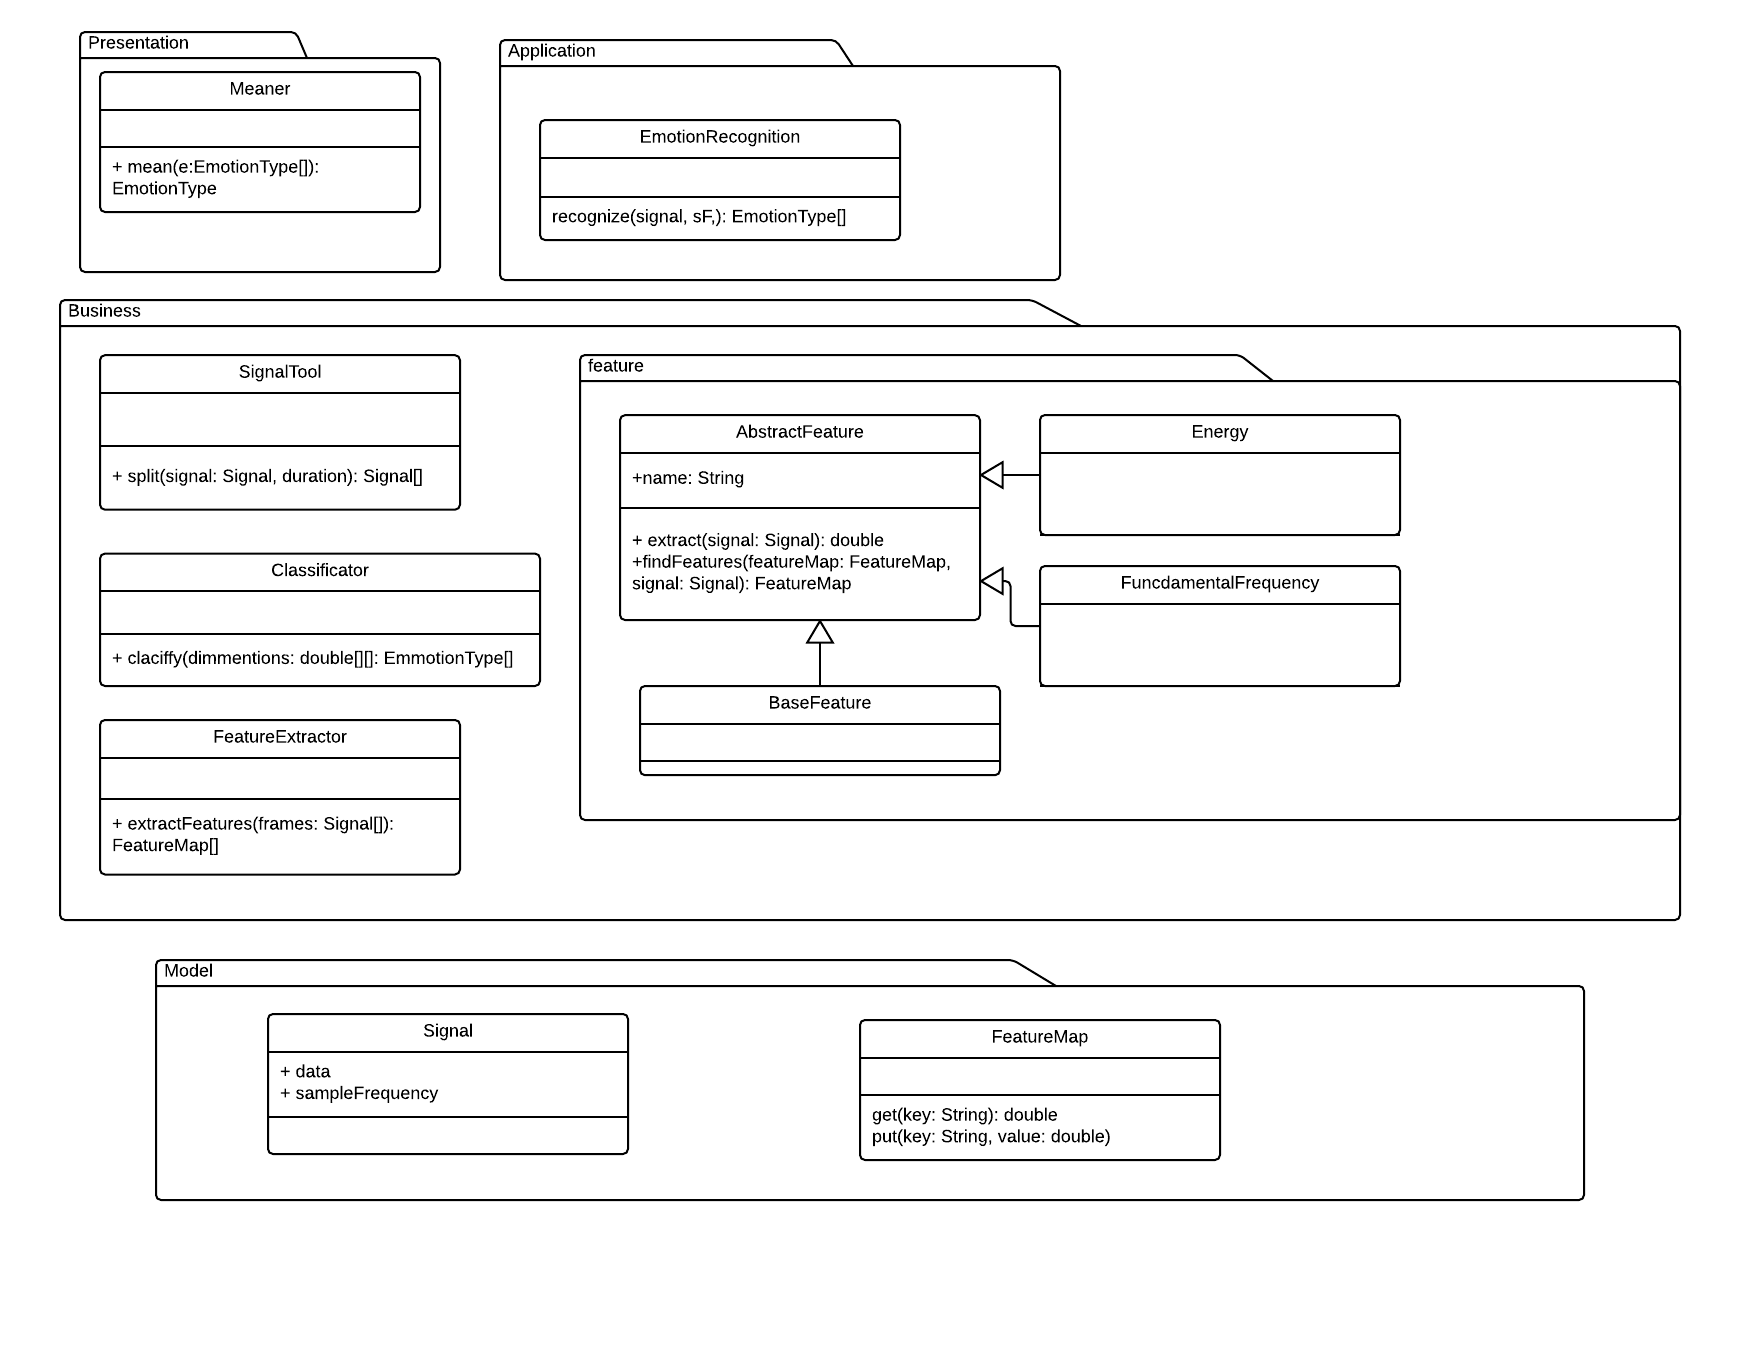
\includegraphics[scale=.4]{diagram_klas}
\end{frame}
\begin{frame}
  \frametitle{Co mam zrobione}
    \begin{itemize}
	\item architekturę(warstwowa)
	\item metodykę(TDD)
	\item model dla sygnału
	\item Mechanizm ekstrakcji cech 
	\item implementację podstawowych cech
    \end{itemize}
\end{frame}
\begin{frame}
  \frametitle{Plan na najbliższą przyszłość}
    \begin{itemize}
	\item podstawowa prezentacja, wykresy
	\item ekstrakcję pozostałych cech
	\item zmiana reprezentacji cech z liczby zmiennoprzecinkowej na ich wektor
    \end{itemize}
\end{frame}
\begin{frame}
  \frametitle{Bieżące problemy}
    \begin{itemize}
	\item nie umiem cyfrowego przetwarzania sygnałów
	\item matlab jest dla mnie nieprzewidywalny
    \end{itemize}
\end{frame}
\end{document}

%%%%%%%%%%%%%%%%%%%%%%%%%%%%%%%%%%%%%%%%%%%%%%%%%%%%%%%%%%%%%%%%%%%%%%%%%%%%%%%%
\begin{frame}
  \frametitle{Jak wygląda większość "programów" w Matlabie?}
  \begin{enumerate}
  \end{enumerate}
\end{frame}
%
%	PREZENTACJA 1
%
\begin{frame}
  \frametitle{Jak człowiek okazuje emocje?}
  \begin{itemize}
    \item mimika
    \item gesty
    \item mowa ciała
    \item reakcje wewnętrzne organizmu
    \item mowa
  \end{itemize}
%https://www.newscientist.com/article/mg22129595-200-feeling-sad-computer-knows-by-looking-at-how-you-move/
\end{frame}
\begin{frame}
  \frametitle{Gdzie się stosuje?}
  \begin{itemize}
    \item nauka rozpoznawania emocji (autyzm)
    \item centra obsługi klienta
    \item rozpoznawanie stanu pacjentów
    \item komputer rozumie emocje człowieka
  \end{itemize}
\end{frame}
\begin{frame}
  \frametitle{Podstawowe emocje}
  \begin{itemize}
    \item radość
    \item smutek
    \item gniew
    \item strach
    \item zdziwienie
    \item zniesmaczenie
  \end{itemize}
\end{frame}
\begin{frame}
  \frametitle{Model Plutchika}
  \begin{itemize}
	\item radość – smutek
	\item złość – strach
	\item oczekiwanie – zaskoczenie
	\item zaufanie – zniesmaczenie
  \end{itemize}
\end{frame}
\begin{frame}
  \frametitle{Model Plutchika - obraz}
    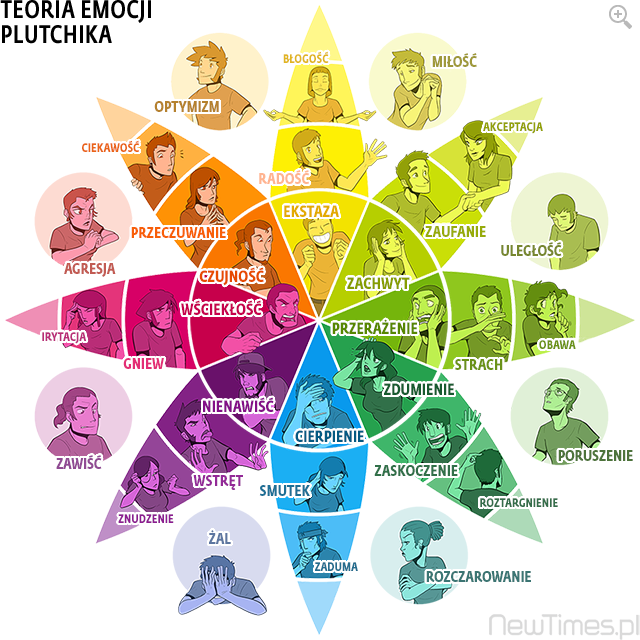
\includegraphics[scale=.4]{plutchik}
\end{frame}
\begin{frame}
  \frametitle{Dla czego mowa?}
  \begin{itemize}
    \item można ją nagrać wszędzie
    \item kamera musi być skierowana na człowieka
    \item twarz, ciało można zasłonić
    \item wystarczy mikrofon
  \end{itemize}
\end{frame}
\begin{frame}
  \frametitle{Różnice między mówcami}
  \begin{itemize}
    \item cechy indywidualne
    \item kultura
    \item środowisko
    \item cechy sygnału % różne cechy u różnych ludzi
  \end{itemize}
\end{frame}
\begin{frame}
  \frametitle{Emocje w przestrzeni dwuwymiarowej}
    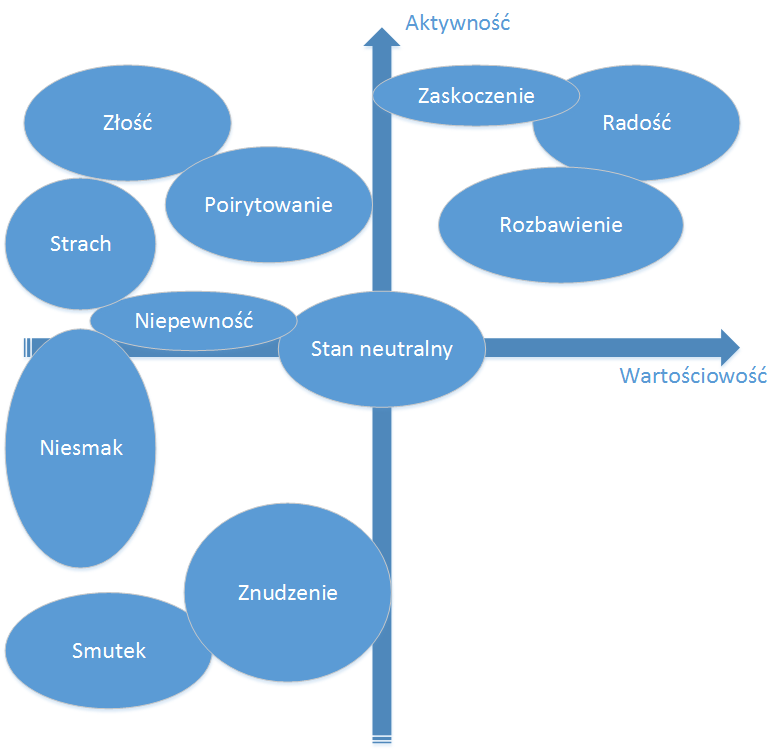
\includegraphics[scale=.25]{dwa_wymiary}
\end{frame}
\begin{frame}
  \frametitle{Klasyfikatory}
  \begin{itemize}
        \item k-najbliższych sąsiadów
	\item metodę drzewa
	\item analizę dyskryminacyjną
	\item ukryte modele Markowa
	\item gusowskie modele mieszane
	\item sztuczne sieci neuronowe
        \item maszynę wektorów wspierających
        \item podejście mieszane
  \end{itemize}
\end{frame}
\begin{frame}
  \frametitle{Bazy mowy}
  \begin{itemize}
    \item spontaniczne
    \item odgrywane
  \end{itemize}
\end{frame}
